\documentclass{article}

\usepackage{graphicx}
\usepackage{amsmath}
\usepackage{xepersian}

\settextfont{Times New Roman}

\title{تمرین سوم طراحی سیستم‌های دیجیتال}
\author{پارسا محمدیان -- 98102284}

\begin{document}
\maketitle
\newpage
\section{طراحی}
در این تمرین از ما خواسته شده  
\lr{RAM} 
طراحی کنیم که پورت 
\lr{data} 
آن دو طرفه یعنی از نوع 
\lr{inout} 
باشد. برای پیاده سازی 
\lr{inout} 
از بافر سه حالته استفاده می‌کنیم.

پیاده‌سازی بافر سه حالته در فایل 
\lr{tri\_state\_buffer.v} 
موجود است. سپس بقیه اجزای حافظه را با ابعاد پارامتریک پیاده‌سازی می‌کنیم. جزئیات پیاده‌سازی در فایل 
\lr{ram.v} 
موجود است.

\section{تست}
برای تست مدار ماژولی در فایل 
\lr{stimulus.v} 
نوشته شده که طول آدرس رم را 4 و طول کلمه رم را 8 بیت قرار می‌دهد. حال ابتدا چندین مقدار در حافظه نوشته شده، 
سپس با آدرس همان مقادیر خوانده شده. با توجه به یکسان بودن مقادیر نوشته شده و خوانده شده به صحت عملکرد حافظه 
پی می‌بریم.

در شکل زیر ابتدا مقدار 8 در خانه صفر حافظه 
نوشته شده است. سپس مقدار 16 در خانه سوم حافظه نوشته شده است. 
پس از آن به سراغ خواندن از حافظه رفته و مقدار خانه 0 را می‌خوانیم که به درستی 
مقدار 8 را دارد. بار دیگر مقدار آدرس 1 را می‌خوانیم که چون 
هیچ مقداری به آن ندادیم مقدار 
\lr{x} 
را دارد. حال دوباره مقدار آدرس 2 را می‌خوانیم که طبق انتظار 16 است و رم به صورت صحیح کار می‌کند.

\begin{figure}[!htbp]
    \centering
    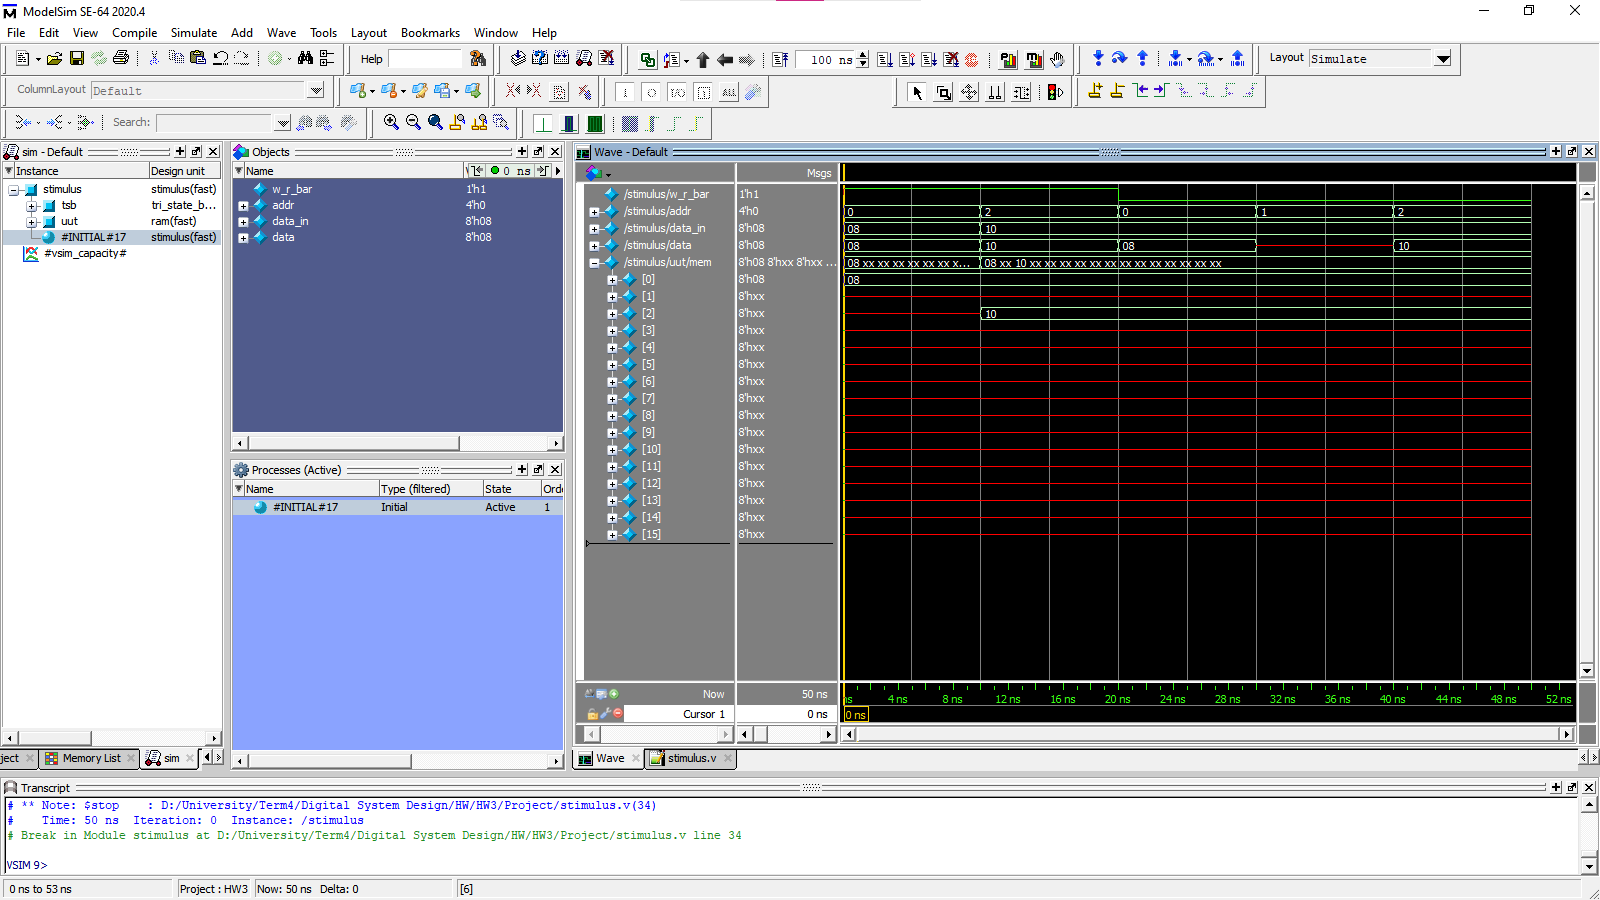
\includegraphics[width=\linewidth]{wave.png}
\end{figure}

\end{document}